%-*-latex-*-
\sectionthree{Notation}
\begin{python0}
from solutions import *; clear()
\end{python0}

Unfortunately probability theory is a big mess with no
standard notation.

Note that it's common to use a random variable also as a pdf.
For instance some books will say
\[
\Pr[B(n,p) = k] = \binom{n}{k} p^kq^{n-k}
\]
i.e., $B(n,p)$ is a r.v.
and also
\[
B(n,p)(k) = \binom{n}{k} p^kq^{n-k}
\]
i.e., as a pdf.
Some books put parameters as subscript:
\[
B_{(n,p)}
\]

\begin{center}
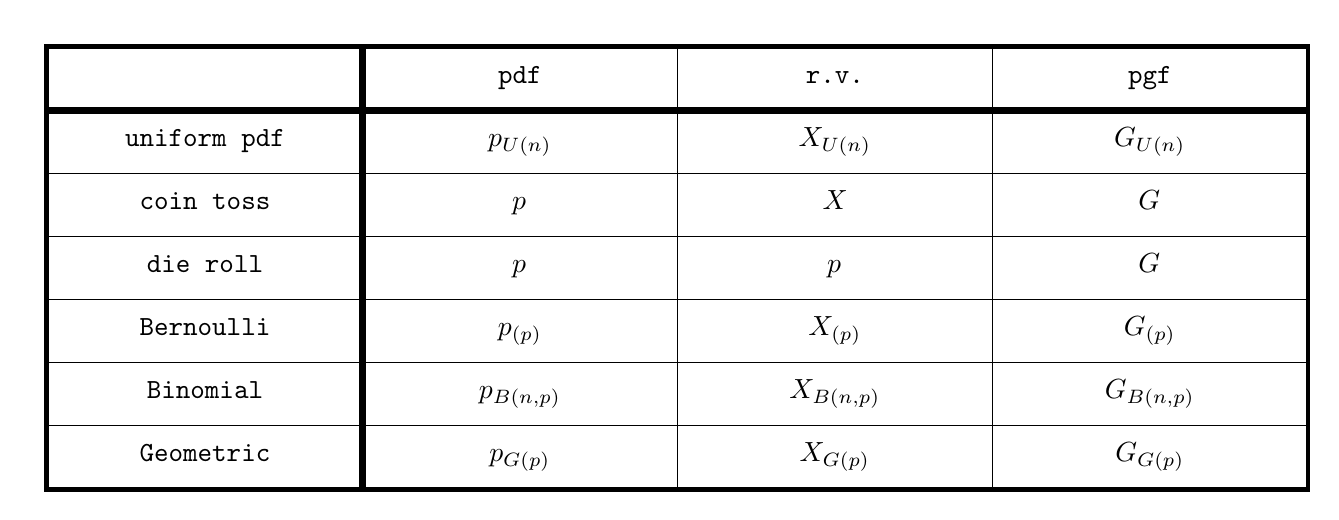
\begin{tikzpicture}

\draw (2.0, -0.4)
  node[draw, line width=0.02cm, , color=black,
       rounded corners=0cm, inner sep=0cm] {

\begin{minipage}[t][0.8cm]{4.0cm}
\mbox{}

\end{minipage}

};\draw (2.0, -0.4) node[color=black] {{\texttt{{\vphantom{pdfr.v.pgfuniform pdfcoin tossdie rollBernoulliBinomialGeometric$p_{U(n)}$$X_{U(n)}$$G_{U(n)}$$p_{\COIN}$$X_{\COIN}$$G_{\COIN}$$p_{\DIE}$$G_{\DIE}$$p_{\BERNOULLI(p)}$$X_{\BERNOULLI(p)}$$G_{\BERNOULLI(p)}$$p_{B(n,p)}$$X_{B(n,p)}$$G_{B(n,p)}$$p_{G(p)}$$X_{G(p)}$$G_{G(p)}$}}}}};\node[anchor=south] at (2.0,0.01) {};\node[anchor=east] at (-0.01,-0.4) {};
\draw (2.0, -0.4)
  node[draw, line width=0.06cm, , color=black,
       rounded corners=0cm, inner sep=0cm] {

\begin{minipage}[t][0.82cm]{4.02cm}
\mbox{}

\end{minipage}

};
\draw (6.0, -0.4)
  node[draw, line width=0.02cm, , color=black,
       rounded corners=0cm, inner sep=0cm] {

\begin{minipage}[t][0.8cm]{4.0cm}
\mbox{}

\end{minipage}

};\draw (6.0, -0.4) node[color=black] {{\texttt{{\vphantom{pdfr.v.pgfuniform pdfcoin tossdie rollBernoulliBinomialGeometric$p_{U(n)}$$X_{U(n)}$$G_{U(n)}$$p_{\COIN}$$X_{\COIN}$$G_{\COIN}$$p_{\DIE}$$G_{\DIE}$$p_{\BERNOULLI(p)}$$X_{\BERNOULLI(p)}$$G_{\BERNOULLI(p)}$$p_{B(n,p)}$$X_{B(n,p)}$$G_{B(n,p)}$$p_{G(p)}$$X_{G(p)}$$G_{G(p)}$}pdf}}}};
\draw (10.0, -0.4)
  node[draw, line width=0.02cm, , color=black,
       rounded corners=0cm, inner sep=0cm] {

\begin{minipage}[t][0.8cm]{4.0cm}
\mbox{}

\end{minipage}

};\draw (10.0, -0.4) node[color=black] {{\texttt{{\vphantom{pdfr.v.pgfuniform pdfcoin tossdie rollBernoulliBinomialGeometric$p_{U(n)}$$X_{U(n)}$$G_{U(n)}$$p_{\COIN}$$X_{\COIN}$$G_{\COIN}$$p_{\DIE}$$G_{\DIE}$$p_{\BERNOULLI(p)}$$X_{\BERNOULLI(p)}$$G_{\BERNOULLI(p)}$$p_{B(n,p)}$$X_{B(n,p)}$$G_{B(n,p)}$$p_{G(p)}$$X_{G(p)}$$G_{G(p)}$}r.v.}}}};
\draw (14.0, -0.4)
  node[draw, line width=0.02cm, , color=black,
       rounded corners=0cm, inner sep=0cm] {

\begin{minipage}[t][0.8cm]{4.0cm}
\mbox{}

\end{minipage}

};\draw (14.0, -0.4) node[color=black] {{\texttt{{\vphantom{pdfr.v.pgfuniform pdfcoin tossdie rollBernoulliBinomialGeometric$p_{U(n)}$$X_{U(n)}$$G_{U(n)}$$p_{\COIN}$$X_{\COIN}$$G_{\COIN}$$p_{\DIE}$$G_{\DIE}$$p_{\BERNOULLI(p)}$$X_{\BERNOULLI(p)}$$G_{\BERNOULLI(p)}$$p_{B(n,p)}$$X_{B(n,p)}$$G_{B(n,p)}$$p_{G(p)}$$X_{G(p)}$$G_{G(p)}$}pgf}}}};\node[anchor=south] at (6.0,0.01) {};\node[anchor=south] at (10.0,0.01) {};\node[anchor=south] at (14.0,0.01) {};\node[anchor=east] at (3.99,-0.4) {};
\draw (10.000000000000002, -0.4)
  node[draw, line width=0.06cm, , color=black,
       rounded corners=0cm, inner sep=0cm] {

\begin{minipage}[t][0.82cm]{12.02cm}
\mbox{}

\end{minipage}

};
\draw (2.0, -1.2000000000000002)
  node[draw, line width=0.02cm, , color=black,
       rounded corners=0cm, inner sep=0cm] {

\begin{minipage}[t][0.8cm]{4.0cm}
\mbox{}

\end{minipage}

};\draw (2.0, -1.2000000000000002) node[color=black] {{\texttt{{\vphantom{pdfr.v.pgfuniform pdfcoin tossdie rollBernoulliBinomialGeometric$p_{U(n)}$$X_{U(n)}$$G_{U(n)}$$p_{\COIN}$$X_{\COIN}$$G_{\COIN}$$p_{\DIE}$$G_{\DIE}$$p_{\BERNOULLI(p)}$$X_{\BERNOULLI(p)}$$G_{\BERNOULLI(p)}$$p_{B(n,p)}$$X_{B(n,p)}$$G_{B(n,p)}$$p_{G(p)}$$X_{G(p)}$$G_{G(p)}$}uniform pdf}}}};
\draw (2.0, -2.0)
  node[draw, line width=0.02cm, , color=black,
       rounded corners=0cm, inner sep=0cm] {

\begin{minipage}[t][0.8cm]{4.0cm}
\mbox{}

\end{minipage}

};\draw (2.0, -2.0) node[color=black] {{\texttt{{\vphantom{pdfr.v.pgfuniform pdfcoin tossdie rollBernoulliBinomialGeometric$p_{U(n)}$$X_{U(n)}$$G_{U(n)}$$p_{\COIN}$$X_{\COIN}$$G_{\COIN}$$p_{\DIE}$$G_{\DIE}$$p_{\BERNOULLI(p)}$$X_{\BERNOULLI(p)}$$G_{\BERNOULLI(p)}$$p_{B(n,p)}$$X_{B(n,p)}$$G_{B(n,p)}$$p_{G(p)}$$X_{G(p)}$$G_{G(p)}$}coin toss}}}};
\draw (2.0, -2.8000000000000003)
  node[draw, line width=0.02cm, , color=black,
       rounded corners=0cm, inner sep=0cm] {

\begin{minipage}[t][0.8cm]{4.0cm}
\mbox{}

\end{minipage}

};\draw (2.0, -2.8000000000000003) node[color=black] {{\texttt{{\vphantom{pdfr.v.pgfuniform pdfcoin tossdie rollBernoulliBinomialGeometric$p_{U(n)}$$X_{U(n)}$$G_{U(n)}$$p_{\COIN}$$X_{\COIN}$$G_{\COIN}$$p_{\DIE}$$G_{\DIE}$$p_{\BERNOULLI(p)}$$X_{\BERNOULLI(p)}$$G_{\BERNOULLI(p)}$$p_{B(n,p)}$$X_{B(n,p)}$$G_{B(n,p)}$$p_{G(p)}$$X_{G(p)}$$G_{G(p)}$}die roll}}}};
\draw (2.0, -3.6)
  node[draw, line width=0.02cm, , color=black,
       rounded corners=0cm, inner sep=0cm] {

\begin{minipage}[t][0.8cm]{4.0cm}
\mbox{}

\end{minipage}

};\draw (2.0, -3.6) node[color=black] {{\texttt{{\vphantom{pdfr.v.pgfuniform pdfcoin tossdie rollBernoulliBinomialGeometric$p_{U(n)}$$X_{U(n)}$$G_{U(n)}$$p_{\COIN}$$X_{\COIN}$$G_{\COIN}$$p_{\DIE}$$G_{\DIE}$$p_{\BERNOULLI(p)}$$X_{\BERNOULLI(p)}$$G_{\BERNOULLI(p)}$$p_{B(n,p)}$$X_{B(n,p)}$$G_{B(n,p)}$$p_{G(p)}$$X_{G(p)}$$G_{G(p)}$}Bernoulli}}}};
\draw (2.0, -4.4)
  node[draw, line width=0.02cm, , color=black,
       rounded corners=0cm, inner sep=0cm] {

\begin{minipage}[t][0.8cm]{4.0cm}
\mbox{}

\end{minipage}

};\draw (2.0, -4.4) node[color=black] {{\texttt{{\vphantom{pdfr.v.pgfuniform pdfcoin tossdie rollBernoulliBinomialGeometric$p_{U(n)}$$X_{U(n)}$$G_{U(n)}$$p_{\COIN}$$X_{\COIN}$$G_{\COIN}$$p_{\DIE}$$G_{\DIE}$$p_{\BERNOULLI(p)}$$X_{\BERNOULLI(p)}$$G_{\BERNOULLI(p)}$$p_{B(n,p)}$$X_{B(n,p)}$$G_{B(n,p)}$$p_{G(p)}$$X_{G(p)}$$G_{G(p)}$}Binomial}}}};
\draw (2.0, -5.199999999999999)
  node[draw, line width=0.02cm, , color=black,
       rounded corners=0cm, inner sep=0cm] {

\begin{minipage}[t][0.8cm]{4.0cm}
\mbox{}

\end{minipage}

};\draw (2.0, -5.199999999999999) node[color=black] {{\texttt{{\vphantom{pdfr.v.pgfuniform pdfcoin tossdie rollBernoulliBinomialGeometric$p_{U(n)}$$X_{U(n)}$$G_{U(n)}$$p_{\COIN}$$X_{\COIN}$$G_{\COIN}$$p_{\DIE}$$G_{\DIE}$$p_{\BERNOULLI(p)}$$X_{\BERNOULLI(p)}$$G_{\BERNOULLI(p)}$$p_{B(n,p)}$$X_{B(n,p)}$$G_{B(n,p)}$$p_{G(p)}$$X_{G(p)}$$G_{G(p)}$}Geometric}}}};\node[anchor=south] at (2.0,-0.79) {};\node[anchor=east] at (-0.01,-1.2000000000000002) {};\node[anchor=east] at (-0.01,-2.0000000000000004) {};\node[anchor=east] at (-0.01,-2.8000000000000003) {};\node[anchor=east] at (-0.01,-3.6) {};\node[anchor=east] at (-0.01,-4.4) {};\node[anchor=east] at (-0.01,-5.199999999999999) {};
\draw (2.0, -3.1999999999999997)
  node[draw, line width=0.06cm, , color=black,
       rounded corners=0cm, inner sep=0cm] {

\begin{minipage}[t][4.82cm]{4.02cm}
\mbox{}

\end{minipage}

};
\draw (6.0, -1.2000000000000002)
  node[draw, line width=0.02cm, , color=black,
       rounded corners=0cm, inner sep=0cm] {

\begin{minipage}[t][0.8cm]{4.0cm}
\mbox{}

\end{minipage}

};\draw (6.0, -1.2000000000000002) node[color=black] {{\texttt{{\vphantom{pdfr.v.pgfuniform pdfcoin tossdie rollBernoulliBinomialGeometric$p_{U(n)}$$X_{U(n)}$$G_{U(n)}$$p_{\COIN}$$X_{\COIN}$$G_{\COIN}$$p_{\DIE}$$G_{\DIE}$$p_{\BERNOULLI(p)}$$X_{\BERNOULLI(p)}$$G_{\BERNOULLI(p)}$$p_{B(n,p)}$$X_{B(n,p)}$$G_{B(n,p)}$$p_{G(p)}$$X_{G(p)}$$G_{G(p)}$}$p_{U(n)}$}}}};
\draw (10.0, -1.2000000000000002)
  node[draw, line width=0.02cm, , color=black,
       rounded corners=0cm, inner sep=0cm] {

\begin{minipage}[t][0.8cm]{4.0cm}
\mbox{}

\end{minipage}

};\draw (10.0, -1.2000000000000002) node[color=black] {{\texttt{{\vphantom{pdfr.v.pgfuniform pdfcoin tossdie rollBernoulliBinomialGeometric$p_{U(n)}$$X_{U(n)}$$G_{U(n)}$$p_{\COIN}$$X_{\COIN}$$G_{\COIN}$$p_{\DIE}$$G_{\DIE}$$p_{\BERNOULLI(p)}$$X_{\BERNOULLI(p)}$$G_{\BERNOULLI(p)}$$p_{B(n,p)}$$X_{B(n,p)}$$G_{B(n,p)}$$p_{G(p)}$$X_{G(p)}$$G_{G(p)}$}$X_{U(n)}$}}}};
\draw (14.0, -1.2000000000000002)
  node[draw, line width=0.02cm, , color=black,
       rounded corners=0cm, inner sep=0cm] {

\begin{minipage}[t][0.8cm]{4.0cm}
\mbox{}

\end{minipage}

};\draw (14.0, -1.2000000000000002) node[color=black] {{\texttt{{\vphantom{pdfr.v.pgfuniform pdfcoin tossdie rollBernoulliBinomialGeometric$p_{U(n)}$$X_{U(n)}$$G_{U(n)}$$p_{\COIN}$$X_{\COIN}$$G_{\COIN}$$p_{\DIE}$$G_{\DIE}$$p_{\BERNOULLI(p)}$$X_{\BERNOULLI(p)}$$G_{\BERNOULLI(p)}$$p_{B(n,p)}$$X_{B(n,p)}$$G_{B(n,p)}$$p_{G(p)}$$X_{G(p)}$$G_{G(p)}$}$G_{U(n)}$}}}};
\draw (6.0, -2.0)
  node[draw, line width=0.02cm, , color=black,
       rounded corners=0cm, inner sep=0cm] {

\begin{minipage}[t][0.8cm]{4.0cm}
\mbox{}

\end{minipage}

};\draw (6.0, -2.0) node[color=black] {{\texttt{{\vphantom{pdfr.v.pgfuniform pdfcoin tossdie rollBernoulliBinomialGeometric$p_{U(n)}$$X_{U(n)}$$G_{U(n)}$$p_{\COIN}$$X_{\COIN}$$G_{\COIN}$$p_{\DIE}$$G_{\DIE}$$p_{\BERNOULLI(p)}$$X_{\BERNOULLI(p)}$$G_{\BERNOULLI(p)}$$p_{B(n,p)}$$X_{B(n,p)}$$G_{B(n,p)}$$p_{G(p)}$$X_{G(p)}$$G_{G(p)}$}$p_{\COIN}$}}}};
\draw (10.0, -2.0)
  node[draw, line width=0.02cm, , color=black,
       rounded corners=0cm, inner sep=0cm] {

\begin{minipage}[t][0.8cm]{4.0cm}
\mbox{}

\end{minipage}

};\draw (10.0, -2.0) node[color=black] {{\texttt{{\vphantom{pdfr.v.pgfuniform pdfcoin tossdie rollBernoulliBinomialGeometric$p_{U(n)}$$X_{U(n)}$$G_{U(n)}$$p_{\COIN}$$X_{\COIN}$$G_{\COIN}$$p_{\DIE}$$G_{\DIE}$$p_{\BERNOULLI(p)}$$X_{\BERNOULLI(p)}$$G_{\BERNOULLI(p)}$$p_{B(n,p)}$$X_{B(n,p)}$$G_{B(n,p)}$$p_{G(p)}$$X_{G(p)}$$G_{G(p)}$}$X_{\COIN}$}}}};
\draw (14.0, -2.0)
  node[draw, line width=0.02cm, , color=black,
       rounded corners=0cm, inner sep=0cm] {

\begin{minipage}[t][0.8cm]{4.0cm}
\mbox{}

\end{minipage}

};\draw (14.0, -2.0) node[color=black] {{\texttt{{\vphantom{pdfr.v.pgfuniform pdfcoin tossdie rollBernoulliBinomialGeometric$p_{U(n)}$$X_{U(n)}$$G_{U(n)}$$p_{\COIN}$$X_{\COIN}$$G_{\COIN}$$p_{\DIE}$$G_{\DIE}$$p_{\BERNOULLI(p)}$$X_{\BERNOULLI(p)}$$G_{\BERNOULLI(p)}$$p_{B(n,p)}$$X_{B(n,p)}$$G_{B(n,p)}$$p_{G(p)}$$X_{G(p)}$$G_{G(p)}$}$G_{\COIN}$}}}};
\draw (6.0, -2.8000000000000003)
  node[draw, line width=0.02cm, , color=black,
       rounded corners=0cm, inner sep=0cm] {

\begin{minipage}[t][0.8cm]{4.0cm}
\mbox{}

\end{minipage}

};\draw (6.0, -2.8000000000000003) node[color=black] {{\texttt{{\vphantom{pdfr.v.pgfuniform pdfcoin tossdie rollBernoulliBinomialGeometric$p_{U(n)}$$X_{U(n)}$$G_{U(n)}$$p_{\COIN}$$X_{\COIN}$$G_{\COIN}$$p_{\DIE}$$G_{\DIE}$$p_{\BERNOULLI(p)}$$X_{\BERNOULLI(p)}$$G_{\BERNOULLI(p)}$$p_{B(n,p)}$$X_{B(n,p)}$$G_{B(n,p)}$$p_{G(p)}$$X_{G(p)}$$G_{G(p)}$}$p_{\DIE}$}}}};
\draw (10.0, -2.8000000000000003)
  node[draw, line width=0.02cm, , color=black,
       rounded corners=0cm, inner sep=0cm] {

\begin{minipage}[t][0.8cm]{4.0cm}
\mbox{}

\end{minipage}

};\draw (10.0, -2.8000000000000003) node[color=black] {{\texttt{{\vphantom{pdfr.v.pgfuniform pdfcoin tossdie rollBernoulliBinomialGeometric$p_{U(n)}$$X_{U(n)}$$G_{U(n)}$$p_{\COIN}$$X_{\COIN}$$G_{\COIN}$$p_{\DIE}$$G_{\DIE}$$p_{\BERNOULLI(p)}$$X_{\BERNOULLI(p)}$$G_{\BERNOULLI(p)}$$p_{B(n,p)}$$X_{B(n,p)}$$G_{B(n,p)}$$p_{G(p)}$$X_{G(p)}$$G_{G(p)}$}$p_{\DIE}$}}}};
\draw (14.0, -2.8000000000000003)
  node[draw, line width=0.02cm, , color=black,
       rounded corners=0cm, inner sep=0cm] {

\begin{minipage}[t][0.8cm]{4.0cm}
\mbox{}

\end{minipage}

};\draw (14.0, -2.8000000000000003) node[color=black] {{\texttt{{\vphantom{pdfr.v.pgfuniform pdfcoin tossdie rollBernoulliBinomialGeometric$p_{U(n)}$$X_{U(n)}$$G_{U(n)}$$p_{\COIN}$$X_{\COIN}$$G_{\COIN}$$p_{\DIE}$$G_{\DIE}$$p_{\BERNOULLI(p)}$$X_{\BERNOULLI(p)}$$G_{\BERNOULLI(p)}$$p_{B(n,p)}$$X_{B(n,p)}$$G_{B(n,p)}$$p_{G(p)}$$X_{G(p)}$$G_{G(p)}$}$G_{\DIE}$}}}};
\draw (6.0, -3.6)
  node[draw, line width=0.02cm, , color=black,
       rounded corners=0cm, inner sep=0cm] {

\begin{minipage}[t][0.8cm]{4.0cm}
\mbox{}

\end{minipage}

};\draw (6.0, -3.6) node[color=black] {{\texttt{{\vphantom{pdfr.v.pgfuniform pdfcoin tossdie rollBernoulliBinomialGeometric$p_{U(n)}$$X_{U(n)}$$G_{U(n)}$$p_{\COIN}$$X_{\COIN}$$G_{\COIN}$$p_{\DIE}$$G_{\DIE}$$p_{\BERNOULLI(p)}$$X_{\BERNOULLI(p)}$$G_{\BERNOULLI(p)}$$p_{B(n,p)}$$X_{B(n,p)}$$G_{B(n,p)}$$p_{G(p)}$$X_{G(p)}$$G_{G(p)}$}$p_{\BERNOULLI(p)}$}}}};
\draw (10.0, -3.6)
  node[draw, line width=0.02cm, , color=black,
       rounded corners=0cm, inner sep=0cm] {

\begin{minipage}[t][0.8cm]{4.0cm}
\mbox{}

\end{minipage}

};\draw (10.0, -3.6) node[color=black] {{\texttt{{\vphantom{pdfr.v.pgfuniform pdfcoin tossdie rollBernoulliBinomialGeometric$p_{U(n)}$$X_{U(n)}$$G_{U(n)}$$p_{\COIN}$$X_{\COIN}$$G_{\COIN}$$p_{\DIE}$$G_{\DIE}$$p_{\BERNOULLI(p)}$$X_{\BERNOULLI(p)}$$G_{\BERNOULLI(p)}$$p_{B(n,p)}$$X_{B(n,p)}$$G_{B(n,p)}$$p_{G(p)}$$X_{G(p)}$$G_{G(p)}$}$X_{\BERNOULLI(p)}$}}}};
\draw (14.0, -3.6)
  node[draw, line width=0.02cm, , color=black,
       rounded corners=0cm, inner sep=0cm] {

\begin{minipage}[t][0.8cm]{4.0cm}
\mbox{}

\end{minipage}

};\draw (14.0, -3.6) node[color=black] {{\texttt{{\vphantom{pdfr.v.pgfuniform pdfcoin tossdie rollBernoulliBinomialGeometric$p_{U(n)}$$X_{U(n)}$$G_{U(n)}$$p_{\COIN}$$X_{\COIN}$$G_{\COIN}$$p_{\DIE}$$G_{\DIE}$$p_{\BERNOULLI(p)}$$X_{\BERNOULLI(p)}$$G_{\BERNOULLI(p)}$$p_{B(n,p)}$$X_{B(n,p)}$$G_{B(n,p)}$$p_{G(p)}$$X_{G(p)}$$G_{G(p)}$}$G_{\BERNOULLI(p)}$}}}};
\draw (6.0, -4.4)
  node[draw, line width=0.02cm, , color=black,
       rounded corners=0cm, inner sep=0cm] {

\begin{minipage}[t][0.8cm]{4.0cm}
\mbox{}

\end{minipage}

};\draw (6.0, -4.4) node[color=black] {{\texttt{{\vphantom{pdfr.v.pgfuniform pdfcoin tossdie rollBernoulliBinomialGeometric$p_{U(n)}$$X_{U(n)}$$G_{U(n)}$$p_{\COIN}$$X_{\COIN}$$G_{\COIN}$$p_{\DIE}$$G_{\DIE}$$p_{\BERNOULLI(p)}$$X_{\BERNOULLI(p)}$$G_{\BERNOULLI(p)}$$p_{B(n,p)}$$X_{B(n,p)}$$G_{B(n,p)}$$p_{G(p)}$$X_{G(p)}$$G_{G(p)}$}$p_{B(n,p)}$}}}};
\draw (10.0, -4.4)
  node[draw, line width=0.02cm, , color=black,
       rounded corners=0cm, inner sep=0cm] {

\begin{minipage}[t][0.8cm]{4.0cm}
\mbox{}

\end{minipage}

};\draw (10.0, -4.4) node[color=black] {{\texttt{{\vphantom{pdfr.v.pgfuniform pdfcoin tossdie rollBernoulliBinomialGeometric$p_{U(n)}$$X_{U(n)}$$G_{U(n)}$$p_{\COIN}$$X_{\COIN}$$G_{\COIN}$$p_{\DIE}$$G_{\DIE}$$p_{\BERNOULLI(p)}$$X_{\BERNOULLI(p)}$$G_{\BERNOULLI(p)}$$p_{B(n,p)}$$X_{B(n,p)}$$G_{B(n,p)}$$p_{G(p)}$$X_{G(p)}$$G_{G(p)}$}$X_{B(n,p)}$}}}};
\draw (14.0, -4.4)
  node[draw, line width=0.02cm, , color=black,
       rounded corners=0cm, inner sep=0cm] {

\begin{minipage}[t][0.8cm]{4.0cm}
\mbox{}

\end{minipage}

};\draw (14.0, -4.4) node[color=black] {{\texttt{{\vphantom{pdfr.v.pgfuniform pdfcoin tossdie rollBernoulliBinomialGeometric$p_{U(n)}$$X_{U(n)}$$G_{U(n)}$$p_{\COIN}$$X_{\COIN}$$G_{\COIN}$$p_{\DIE}$$G_{\DIE}$$p_{\BERNOULLI(p)}$$X_{\BERNOULLI(p)}$$G_{\BERNOULLI(p)}$$p_{B(n,p)}$$X_{B(n,p)}$$G_{B(n,p)}$$p_{G(p)}$$X_{G(p)}$$G_{G(p)}$}$G_{B(n,p)}$}}}};
\draw (6.0, -5.199999999999999)
  node[draw, line width=0.02cm, , color=black,
       rounded corners=0cm, inner sep=0cm] {

\begin{minipage}[t][0.8cm]{4.0cm}
\mbox{}

\end{minipage}

};\draw (6.0, -5.199999999999999) node[color=black] {{\texttt{{\vphantom{pdfr.v.pgfuniform pdfcoin tossdie rollBernoulliBinomialGeometric$p_{U(n)}$$X_{U(n)}$$G_{U(n)}$$p_{\COIN}$$X_{\COIN}$$G_{\COIN}$$p_{\DIE}$$G_{\DIE}$$p_{\BERNOULLI(p)}$$X_{\BERNOULLI(p)}$$G_{\BERNOULLI(p)}$$p_{B(n,p)}$$X_{B(n,p)}$$G_{B(n,p)}$$p_{G(p)}$$X_{G(p)}$$G_{G(p)}$}$p_{G(p)}$}}}};
\draw (10.0, -5.199999999999999)
  node[draw, line width=0.02cm, , color=black,
       rounded corners=0cm, inner sep=0cm] {

\begin{minipage}[t][0.8cm]{4.0cm}
\mbox{}

\end{minipage}

};\draw (10.0, -5.199999999999999) node[color=black] {{\texttt{{\vphantom{pdfr.v.pgfuniform pdfcoin tossdie rollBernoulliBinomialGeometric$p_{U(n)}$$X_{U(n)}$$G_{U(n)}$$p_{\COIN}$$X_{\COIN}$$G_{\COIN}$$p_{\DIE}$$G_{\DIE}$$p_{\BERNOULLI(p)}$$X_{\BERNOULLI(p)}$$G_{\BERNOULLI(p)}$$p_{B(n,p)}$$X_{B(n,p)}$$G_{B(n,p)}$$p_{G(p)}$$X_{G(p)}$$G_{G(p)}$}$X_{G(p)}$}}}};
\draw (14.0, -5.199999999999999)
  node[draw, line width=0.02cm, , color=black,
       rounded corners=0cm, inner sep=0cm] {

\begin{minipage}[t][0.8cm]{4.0cm}
\mbox{}

\end{minipage}

};\draw (14.0, -5.199999999999999) node[color=black] {{\texttt{{\vphantom{pdfr.v.pgfuniform pdfcoin tossdie rollBernoulliBinomialGeometric$p_{U(n)}$$X_{U(n)}$$G_{U(n)}$$p_{\COIN}$$X_{\COIN}$$G_{\COIN}$$p_{\DIE}$$G_{\DIE}$$p_{\BERNOULLI(p)}$$X_{\BERNOULLI(p)}$$G_{\BERNOULLI(p)}$$p_{B(n,p)}$$X_{B(n,p)}$$G_{B(n,p)}$$p_{G(p)}$$X_{G(p)}$$G_{G(p)}$}$G_{G(p)}$}}}};\node[anchor=south] at (6.0,-0.79) {};\node[anchor=south] at (10.0,-0.79) {};\node[anchor=south] at (14.0,-0.79) {};\node[anchor=east] at (3.99,-1.2000000000000002) {};\node[anchor=east] at (3.99,-2.0000000000000004) {};\node[anchor=east] at (3.99,-2.8000000000000003) {};\node[anchor=east] at (3.99,-3.6) {};\node[anchor=east] at (3.99,-4.4) {};\node[anchor=east] at (3.99,-5.199999999999999) {};
\draw (10.000000000000002, -3.1999999999999997)
  node[draw, line width=0.06cm, , color=black,
       rounded corners=0cm, inner sep=0cm] {

\begin{minipage}[t][4.82cm]{12.02cm}
\mbox{}

\end{minipage}

};
\end{tikzpicture}

\end{center}


